\subsubsection{Integrity \& Accountability}\label{sec:integrity}
\begin{figure}[h]
	\centering
	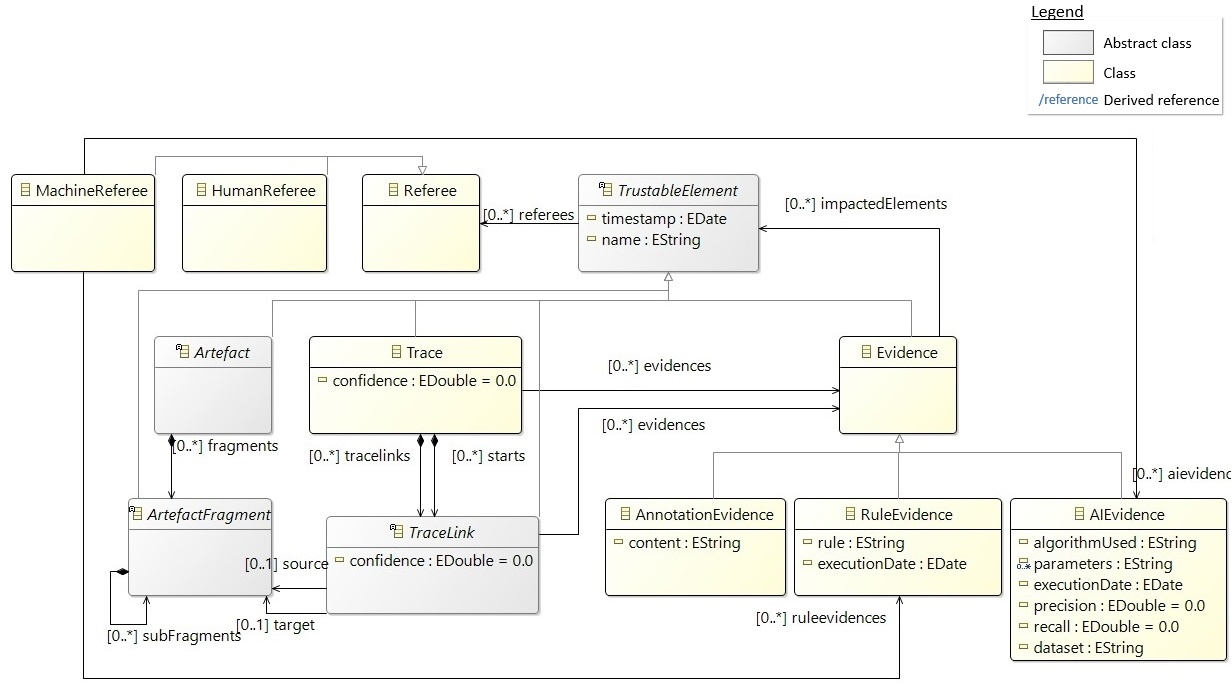
\includegraphics[width=.99\linewidth]{images/integrity.jpg}
	\caption{Integrity}
	\label{fig:mm-integrity}
\end{figure}

When looking at traces is critical to be able to answer questions like "Who is responsible for the creation of this trace?"; "To whom should I refer for more information?"; "How much can I trust this trace is correct?",... If a clear answer is not available, we may lose faith in the whole traceability system or make wrong assumptions on the traceability data that could have very negative impact on the future evolution analysis of the system. 

This is why we believe an explainability mechanism should be a first-class citizen in any traceability approach ~\cite{gotel1995-contribution-structures-req-eng}. Therefore, Tracea brings a dedicated approach to collect, structure, and handle this information.

To begin with, every elements of the Tracea metamodel extends a \texttt{TrusteableElement} (see Figure~\ref{fig:mm-integrity}) as we have seen before. A \texttt{TrusteableElement} contains references to \texttt{Referees} accountable for this element, together with a unique name, and a timestamp.

Beyond this basic support, we also collect evidences for each trace that explain how (and based on what information) that specific trace was created. As such, the \texttt{Evidence} metaclass enables expressing the sets of facts that testify on the means of elicitation, creation, or modification of each elements of a trace. A \texttt{Trace} is potentially linked to a set of evidences. \texttt{Evidence}s are specialized in three subclasses. A trace could be generated as a result of the analysis of a  text annotations with unstructured or grammar-based text explaining the rationale behind such trace (\texttt{AnnotationEvidence}). Or it could be the result of executing a rule (\texttt{RuleEvidence}). Finally, traces can also be the result of the execution of machine learning algorithms and store the type, the ID of the training set, and the precision and recall obtained on that set (\texttt{AIEvidence}).

\texttt{Evidences} increase our certitude that the trace actually exists. Yet, some uncertainty may remind that reflects our belief. We model the (un)certainty a user may have on the quality/existence of the traces with a \textit{confidence} attribute for \texttt{Traces} and \texttt{TraceLinks}. It is a first representation of all the levels of uncertainty that can affect traces (more details in \cite{burgueno2019-uncertainty}).

\paragraph{Classes}
\begin{itemize}
    \item An \textbf{\texttt{Evidence}} is an element that participate in the evaluation of trace reliability. An \texttt{Evidence} references a set of impacted \texttt{TrusteableElements}.
    \item An \texttt{AIEvidence} is an \texttt{Evidence} based on the parameterization and learning precision and recall of an AI algorithm. For example, with traces automatically identified using a machine learning algorithm, an evidence contains the type of the algorithm, its parameters and the level of confidence (\textit{i.e.,} precision and recall on a test bench).
    \item A \texttt{RuleEvidence} is an \texttt{Evidence} describing the execution of integrity rules and their results with a bond to the elements they impact.
    \item An \textbf{\texttt{AnnotationEvidence}}: Textual annotation accounting for Evidence.
    \item A \texttt{Referee} is an actor accountable for a \texttt{TrusteableElement}.
    \item A \texttt{MachineReferee} is a non-human actor responsible for a \texttt{TrusteableElement} (\textit{i.e., } when generated or derived automatically).
    \item A \texttt{HumanReferee}  is a  human actor responsible for a \texttt{TrusteableElement}.
\end{itemize}

\paragraph{Constraints}
No constraints.

\paragraph{Illustrative example}
In our example, \texttt{PoSs} are extracted from certification \texttt{TextDocuments} using natural language processing (NLP) techniques. A \texttt{PoS2NamedEntity} links a \texttt{PoS} and a \texttt{NamedEntity} based on the evaluation of their semantics using machine learning techniques as well. These methods need to be adapted and parameterized, and concrete datasets must be used to train the learning models. We store these attributes in instances of \texttt{AIEvidence} classes. These records will help understand the evolution of the automation.
\begin{figure}[h]
	\centering
	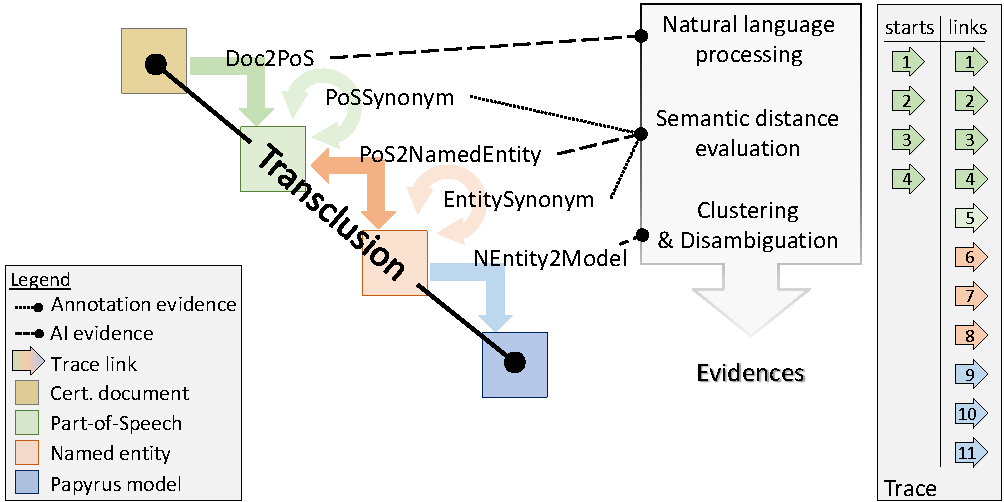
\includegraphics[width=.85\linewidth]{images/relationtyping-re}
	\caption{Complete transclusion process and the record of evidences.}
	\label{fig:mm-relationtyping-re}
\end{figure}
As can be seen in Figure~\ref{fig:mm-relationtyping-re}, we instantiate \texttt{AnnotationEvidence} to record the nature of the synonymy between \texttt{PoSs} and between \texttt{NamedEntities}. 
A \texttt{PoSSynonym} (resp. \texttt{NamedEntitySynonym}) relates two (or more) \texttt{PoS} (reps. \texttt{NamedEntity}) and record the provenance of the evaluation of the distance between the set of elements at play. 

\texttt{Referees} are created for each \texttt{Artifact} and \texttt{Trace} instantiated or modified. The name and the timestamp will provide the useful information to retrieve who is responsible for these elements.


